\section{Obstacle Aware Passivity} \label{sec:obstacle_aware_passivity}
We propose a novel controller, which ensures passivity as defined in \eqref{eq:control_command} but adapts the damping matrix given in \eqref{eq:damping_matrix} based on the desired velocity $\dot{\vecs \xi}$ and obstacles in the surrounding. 
Far away from obstacles, the system is designed to follow the initial velocity, but approaching the obstacle increases the damping, decreasing the chance of a collision.

\ifthesis
\begin{figure}
\centerline{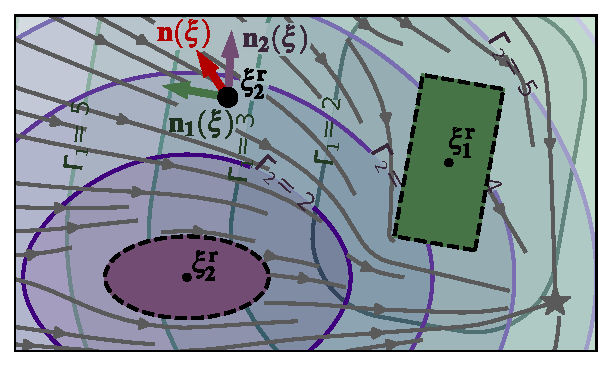
\includegraphics[width=0.7\columnwidth]{figures/normal_and_gamma_field_visualization_annotated.pdf}}
\caption{
The $\Gamma$-field is defined individually for each of the obstacles. At each position $\vecs \xi$, we can evaluate the surface normal $\vect n(\vecs \xi)$. 
The velocity $\vect f(\vecs \xi)$ (gray) avoids collision with the obstacles and converges towards the attractor (star).}
\label{fig:resultant_normal}
\end{figure}
\fi


Hence, the damping matrix $\matd D(\vecs\xi) \in \mathbb{R}^{N \times N}$ smoothly changes from being aligned with the direction of the velocity, as used in \cite{kronander2015passive}, to be aligned with the averaged normal of the obstacles. The desired damping matrix transitions between velocity preserving and collision avoidance using a smoothly defined linear combination:
\begin{equation}
    \matd D(\vecs\xi) = \left(1 - w(\vecs\xi) \right) {\matd D^{f}}(\vecs\xi) + w(\vecs\xi)  {\matd D^{\mathrm{obs}}}(\vecs\xi) \label{eq:damping_summation}
\end{equation}

The danger weight $w(\vecs\xi) \in [0, 1]$ indicates the proximity to the obstacles based on the distance function $\Gamma_o(\vecs \xi)$. Far away from obstacles the weight reaches $w(\vecs \xi) = 0$, whereas $w(\vecs \xi) = 1$ when approaching a boundary:
\begin{equation}
  \begin{split}
w(\vecs\xi) =
\max \left(0,  \frac{\Gamma^{\mathrm{crit}} - \Gamma(\vecs\xi)}{\Gamma^{\mathrm{crit}} - 1} \right) \| \vecs n(\vecs \xi) \| \\
\text{with} \quad
\Gamma(\vecs\xi) = \min_{o = 1..N^{\mathrm{obs}}} \Gamma_o(\vecs\xi)
\label{eq:weight_function}
\end{split}
\end{equation}
The critical distance $\Gamma^{\mathrm{crit}} \in \mathbb{R}_{>0}$ defines the distance where the system has higher damping towards the obstacle.
${\matd D^f}(\vecs\xi)$ and $\matd {D^{\mathrm{obs}}}(\vecs\xi)$ follow design given in \eqref{eq:damping_matrix} and are positive definite matrices, thus $\matd {D}(\vecs\xi)$ is positive definite, too.

\begin{figure}
  \center
  \includesvg[width=0.7\columnwidth]{figures/damping_basis_construction.svg}
\caption{The damping matrix enforcing desired velocity following $\matd{D}^{f}$ has the first basis vector $\vect q_1^{f}$ which points along the avoidance velocity $\vect f(\vecs \xi)$. The damping matrix to enforce collision avoidance $\matd{D}^{\mathrm{obs}}$ uses the normal $\vect n(\vecs \xi)$ to construct the first direction of the decomposition basis $\vect q^{\mathrm{obs}}_1$.}
\label{fig:damping_basis_construction}
%% \label{fig_basis_3D_DS_obs}
\end{figure}

\subsection{Damping for Collision Repulsion} \label{sec:obstacle_repulsion}

\subsubsection{Normal Direction}
The damping matrix $\matd D^{\mathrm{obs}}(\vecs \xi)$ rejects velocities in the direction of the obstacles. To allow this, we introduce an averaged normal direction:
\begin{equation}
  \vecs n(\vecs\xi) = \sum_{o=1}^{N^{\mathrm{obs}}} \vecs{n_o}(\vecs\xi)
  \frac{1 / (\Gamma_o(\vecs \xi) - 1)}{\sum_{p=1}^{N^\mathrm{obs}} 1 / (\Gamma_p(\vecs \xi) - 1)}
  \label{eq:averaged_normal}
\end{equation}
 where the unit normals $\vecs{n_o} (\vecs\xi)$ pointing away from the obstacle $o = 1,  ..,  N^{\mathrm{obs}}$ and are perpendicular to the surface, see Figure~\ref{fig:resultant_normal}. 

The averaged normal $\vecs n(\vecs \xi)$ is a weighted linear combination of the obstacles' normals, giving more importance to closer obstacles.
Additionally, the averaged normal converges to an obstacle normal as we converge towards it, i.e., $\lim_{\Gamma_o(\vecs \xi) \rightarrow 1} \vecs n(\vecs \xi) = \vecs n_o(\vecs \xi)$.
Note that the averaged normal is a zero-vector when two obstacles oppose each other. 

\subsubsection{Decomposition Matrix}
The decomposition matrix $\matd Q^{\mathrm{obs}}(\vecs \xi)$ has its first vector aligned with the normal to the obstacle:  
\begin{equation}
    \vecs q_1^{\mathrm{obs}}(\vecs\xi) =  \vecs n(\vecs\xi) / \lVert\vecs n(\vecs\xi)\rVert 
    \quad \forall \, \xi : \lVert\vecs n(\vecs\xi)\rVert  > 0
\end{equation}
In the case that $\lVert\vecs n(\vecs\xi)\rVert = 0$, the danger weight $w(\vecs \xi)$ from \eqref{eq:weight_function} reaches 0. Hence, the obstacle-aware damping in \eqref{eq:damping_summation} has no effect and is not evaluated.

The second vector is set to be aligned with the desired velocity as much as possible, allowing increased velocity following (Fig.~\ref{fig:damping_basis_construction}). However, it has to remain orthonormal to $\vect q_1^{\mathrm{obs}}$
\begin{equation}
  \vecs q_2^{\mathrm{obs}} = \frac{\hat{\vecs q}_2^{\mathrm{obs}}}{\| \hat{\vecs q}_2^{\mathrm{obs}} \|}
  \quad
  \hat{\vecs q}_2^{\mathrm{obs}} = \vecs q_1^{f} - \vecs q_1^{\mathrm{obs}} p \quad  \forall \, \vecs \xi : | p | < 1
\end{equation}
where velocity unit vector $\vecs q_1^{f}$ is defined in \eqref{eq:velocity_unit_vector}, and the object weight is evaluated as $p = \dotprod{\vecs q_1^{\mathrm{obs}}}{\vecs q_1^{f}}$. 
For the case that $| p | = 1$, the second basis $\vecs q_2^{\mathrm{obs}}$ is set to be any orthonormal vector. The remaining vectors $\vecs q_i^{\mathrm{obs}}, i = 3, .., N$ are constructed to form an orthonormal basis to the first two.

\subsubsection{Damping Values}
Analogously, we smoothly define the values of the diagonal matrix $\matd{S}^{\mathrm{obs}}(\vecs \xi)$:
\begin{equation}
  \matd{S}_d^{\mathrm{obs}}(\vecs \xi) =
  \begin{cases}
    s^{\mathrm{obs}} & d = 1 \\
    | p | s^c + (1 - | p |) s^{f} & d = 2 \\
    s^c & d \geq 3 
  \end{cases}
  \quad d = 1 .. N\
\end{equation}
where the damping along the nominal direction $s^{f} \in \mathbb{R}_{>0}$, obstacle-damping $s^{\mathrm{obs}} \in \mathbb{R}_{>0}$, and the compliant-damping $s^c \in \mathbb{R}_{>0}$ are user-defined parameters which determine the behavior of the passive-controller. The first entry of $\matr{S}^{\mathrm{obs}}$ dictates the damping towards the obstacle, and the second entry the desired velocity following. Note how the second value approaches the compliant damping, as normal and velocity become parallel.

\subsubsection{Damping Only Towards Obstacle} \label{sec:damping_only_toward}
In the presence of an obstacle, the disturbances should be damped strongly when the agent is pushed against the obstacle. Conversely, the system can remain compliant if the motion is away from the obstacle. This is achieved by setting updating the first damping value $\matd{S}^{\mathrm{obs}}_1$ if the robot is moving away from the surface, i.e., $\vecs{\dot\xi}^T \vecs n(\vecs\xi) > 0$:
\begin{equation}
  \matd{S}_1^{\mathrm{obs}} (\vecs \xi) =
  \begin{cases}
    s^{\mathrm{obs}} & \text{if} \;\; \left(\vect f(\vecs \xi) - \vecs{\dot \xi} \right)^T \vecs n(\vect \xi) > 0 \\
    s^{\mathrm{c}} & \text{otherwise}
  \end{cases}
  \label{eq:leaving_compliance}
\end{equation}

\subsection{Damping for Velocity Preservation}
The decomposition matrix $\matd Q^{f}$ is an orthonormal basis with the first vector being parallel to the desired velocity $\vect f(\vecs\xi)$, as proposed in Section~\ref{sec:trad_passive}. Hence, the values of the diagonal matrix $\matd S^{f}$ are high in the direction of the desired velocity (first component), but more compliant in the remaining directions. 
Moreover, the damping is set to ensure that when passing a narrow passage between two obstacles, where the normal vector cancels $\vect n(\vecs \xi) \approx 0\vect 0$, with additionally a low distance value $\Gamma(\vecs \xi) \approx 1$, the damping perpendicular to the velocity direction is high. Hence, we set:
\begin{equation}
  \begin{split}
  \matd{S}^{f}_{d} =
  \begin{cases}
    s^{f} & d = 1 \\
    w^p s^{\mathrm{obs}} + (1- w^p) s^s & d \geq 2 
  \end{cases} \quad d = 1 .. N\\
  \text{with} \quad
  %w^p = \min \left(1,  \| \vecs n(\vecs \xi) \|^2 + \left(\frac{\Gamma(\vecs \xi) -1}{\Gamma^{\mathrm{crit}} - 1}\right) ^2 \right)
   w^p = \min \left(1,  \| \vecs n(\vecs \xi) \|^2 + \left(\frac{\Gamma^{\mathrm{crit}} -\Gamma(\vecs \xi)}{\Gamma^{\mathrm{crit}} - 1}\right) ^2 \right)
  \end{split}
\end{equation}

\subsection{Damping Parameter Design}
Higher values for the damping parameters $s^{(\cdot})$ generally result in improved velocity following and disturbance repulsion, whereas lower values allow more compliant behavior.
The damping value in the direction of the obstacle is set high $s^{\mathrm{obs}}$ to ensure obstacle avoidance even in the presence of high disturbances. 
Conversely, the damping in the direction of the velocity $s^{f}$ is set medium to high, as the system should follow the desired velocity $\vect f(\vecs \xi)$. However, it should remain compliant if needed.
Finally, to facilitate interaction, a low damping value $s^{c}$ should be chosen for all other directions.
This can be summarized as:
\begin{equation}
s^{\mathrm{obs}} > s^{f} \gg s^{c} > 0
\end{equation}
